% !TEX program = lualatex
\documentclass[12pt,a4paper]{ltjsarticle}
\usepackage{amsmath,amssymb,amsthm}
\usepackage{geometry}
\geometry{margin=2.5cm}
\usepackage{hyperref}
\hypersetup{colorlinks=true,linkcolor=blue,citecolor=blue,urlcolor=blue}
\usepackage{booktabs}
\usepackage{luatexja-fontspec}
\usepackage{graphicx}

\title{ディレイ回路モデルでの単振動・正弦波モデルの実現方法}
\author{木原 範昭（Noriaki Kihara）\\
WF System Co., Ltd.\\
大阪大学 基礎工学部 卒業}
\date{2026年4月\quad 研究ノート\\[4pt]
DOI: \href{https://doi.org/10.5281/zenodo.19534349}{10.5281/zenodo.19534349}}

\begin{document}

\maketitle

\begin{abstract}
前稿~\cite{ref1}で構成したディレイ回路モデルは，クラス $A = \{I, \overline{I}\}$ と反転（NOT）演算のみを用いたため，矩形波の振動しか表現できなかった．本稿では，前稿~\cite{ref2}で導入したスーパークラス，メタ情報，演算ファンクション $*$ の枠組みを用いて，クラスの情報と $*$ 演算を具体的に定義することにより，正弦波（横波），縦波，旋回波を実現する．いずれの場合も，ディレイ回路 $F_D$ および NOT演算回路の定義は変更せず，クラスの定義と演算ファンクション $*$ の選択のみで異なる波動パターンが得られることを示す．
\end{abstract}

\section{はじめに}

前稿~\cite{ref1}では，クラス $A = \{I, \overline{I}\}$ と反転（NOT）演算のみを用いて，離散的な矩形波振動を構成した．前稿~\cite{ref2}では，スーパークラス，メタ情報（カウンタ $n$，演算ファンクション $*$），および $F_D$ の拡張定義を導入した．

本稿では，\cite{ref2}の枠組みを用いて，クラス $A$ の情報，メタ情報，および演算ファンクション $*$ を具体的に定義することにより，正弦波（縦波・横波・旋回波）を実現するモデルを構成する．

\section{準備：前稿の定義の要約}

本稿は，前稿~\cite{ref1}で定義したディレイ回路 $F_D$，NOT演算回路，および情報 $I$ の性質（null 状態，等価判定，反転）を前提とする．また，前稿~\cite{ref2}で導入した以下の概念を用いる：

\begin{itemize}
  \item \textbf{スーパークラス}：異なるクラスに属する情報の組 $(A, B, C_1, \ldots, C_m)$（\cite{ref2} \S 3.2）
  \item \textbf{メタ情報}：カウンタ $n$（ディレイ回数）および演算ファンクション $*$（\cite{ref2} \S 3.2）
  \item \textbf{$F_D$ の拡張定義}：$F_D$ 通過時にカウンタ $n$ をインクリメントし，$*$ が $\mathrm{null}$ でなければ実行する（\cite{ref2} \S 3.3）
\end{itemize}

これらの定義の詳細は各前稿を参照されたい．

\section{単振動クラス $A$ の定義}

\subsection{前稿における単振動回路}

前稿~\cite{ref1} \S 3 において，ディレイ回路 $F_D$ とNOT演算回路を接続し，以下の帰還構造を構成した．$F_D$ の出力を NOT の入力に，NOT の出力を $F_D$ の入力に接続する．

\begin{figure}[htbp]
  \centering
  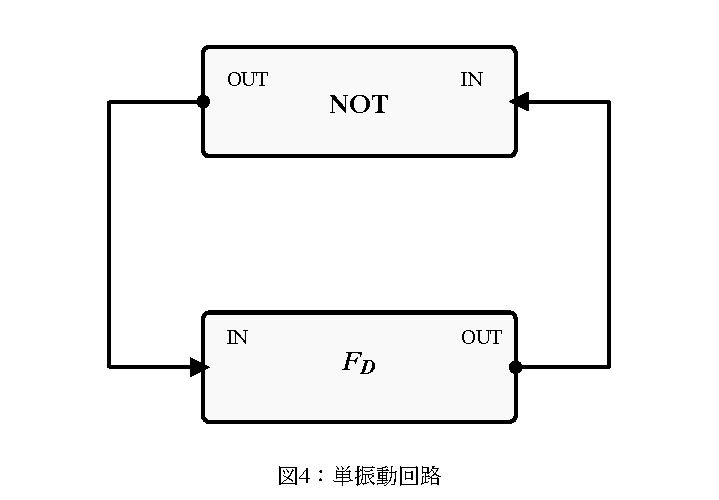
\includegraphics[width=0.6\textwidth]{fig4_oscillation_circuit.pdf}
  \caption{単振動回路（\cite{ref1} 図4 再掲）}
  \label{fig:oscillation_circuit}
\end{figure}

単振動回路の各回における出力の遷移を以下に示す．

\begin{table}[htbp]
  \centering
  \begin{tabular}{ccc}
    \toprule
    ディレイ回数 $n$ & $F_D$ の OUT & NOT の OUT \\
    \midrule
    0 & $\mathrm{null}$ & $\mathrm{null}$ \\
    1 & $I$ & $\overline{I}$ \\
    2 & $\overline{I}$ & $I$ \\
    3 & $I$ & $\overline{I}$ \\
    4 & $\overline{I}$ & $I$ \\
    $\vdots$ & $\vdots$ & $\vdots$ \\
    \bottomrule
  \end{tabular}
\end{table}

$n \geq 1$ において，$F_D$ の出力は $I$ と $\overline{I}$ を交互に繰り返す．これは離散的な振動である．

情報 $I$ をスカラー値とし，反転を $\overline{I} = -I$ と定めると，単振動回路の $F_D$ の出力は次のように表される：

\begin{equation}
x(n) = I \cdot (-1)^{n+1} \quad (n = 1, 2, 3, \ldots)
\end{equation}

すなわち，出力はディレイ回数 $n$ に対して $I$ と $-I$ を交互に繰り返す．これは矩形波である．

\subsection{矩形波のクラス $A$ の定義}

前稿~\cite{ref2}の枠組みにおいて，\S 3.1 の矩形波振動を再定義する．

\begin{itemize}
  \item \textbf{クラス $A$ の情報}：スカラー値 $i$
  \item \textbf{メタ情報}：$\mathrm{null}$（カウンタ $n$，演算ファンクション $*$ ともに不要）
\end{itemize}

反転は NOT演算回路により $\overline{i} = -i$ として与えられる．メタ情報が $\mathrm{null}$ であるため，$F_D$ 通過時に追加の演算は実行されず，\S 3.1 の単振動回路と同一の結果を与える．

\begin{equation}
x(n) = i \cdot (-1)^{n+1} \quad (n = 1, 2, 3, \ldots)
\end{equation}

\subsection{矩形波のクラス $A$ による伝播と振動}

\S 3.2 で定義した矩形波のクラス $A$（スカラー値 $i$，メタ情報 $\mathrm{null}$）を，前稿~\cite{ref1} \S 4 の開いた縄モデルおよび \S 5 の閉じた縄モデルに適用する．

メタ情報が $\mathrm{null}$ であるため，$F_D$ 通過時に追加の演算は実行されない．$F_D$ の基本演算規則（入力情報を内部にコピーし，1ステップの遅延の後に出力する）のみが動作する．

したがって，開いた縄モデルでは情報 $i$ が各 $F_D$ を1ステップずつそのまま通過し，\cite{ref1} \S 4 と同一の伝播シーケンス（到達位置 $k = n$）を与える．閉じた縄モデルでは，NOT演算回路による反転を含め，\cite{ref1} \S 5 と同一の振動シーケンス（1振動 $= 2n$ 回の演算）を与える．

すなわち，矩形波のクラス $A$ は，前稿~\cite{ref1}の全構成（単振動回路，開いた縄，閉じた縄）の結果をそのまま再現する．

\subsection{横波のクラス $B$ の定義}

横波を実現するクラス $B$ を以下のように定義する．

\textbf{クラス $B$ の情報：}

\begin{itemize}
  \item $i$：スカラー値（入力値．クラス $A$ と同一）
  \item $w$：実数値（振幅．出力用）
\end{itemize}

\textbf{メタ情報：}

\begin{itemize}
  \item $n$：カウンタ（ディレイ回数．\cite{ref2} \S 3.3 の定義による）
  \item $m$：波長に相当するディレイ回数（$1, 2, 3, \ldots$ の正の整数）
\end{itemize}

\textbf{演算ファンクション $*$：}

\begin{equation}
w = i \cdot \sin\!\left(\frac{n}{m} \cdot 360{}^\circ\right)
\end{equation}

$F_D$ を通過するたびに $n$ がインクリメントされ，演算ファンクション $*$ が実行されて $w$ が更新される．出力 $w$ を観測すれば，ディレイ回数 $n$ の進行に伴い正弦波的な振動を得る．

\subsection{クラス $B$ の振動シーケンス}

$i = 1$，$m = 12$ の場合，単振動回路における $F_D$ の出力 $w$ の遷移を以下に示す．

\begin{table}[htbp]
  \centering
  \begin{tabular}{ccc}
    \toprule
    ディレイ回数 $n$ & $n/m \cdot 360{}^\circ$ & $w = \sin(n/m \cdot 360{}^\circ)$ \\
    \midrule
    0  & $0{}^\circ$   & 0.000 \\
    1  & $30{}^\circ$  & 0.500 \\
    2  & $60{}^\circ$  & 0.866 \\
    3  & $90{}^\circ$  & 1.000 \\
    4  & $120{}^\circ$ & 0.866 \\
    5  & $150{}^\circ$ & 0.500 \\
    6  & $180{}^\circ$ & 0.000 \\
    7  & $210{}^\circ$ & $-0.500$ \\
    8  & $240{}^\circ$ & $-0.866$ \\
    9  & $270{}^\circ$ & $-1.000$ \\
    10 & $300{}^\circ$ & $-0.866$ \\
    11 & $330{}^\circ$ & $-0.500$ \\
    12 & $360{}^\circ$ & 0.000 \\
    \bottomrule
  \end{tabular}
\end{table}

$n = 12$ で1周期が完了し，以降は同じパターンを繰り返す．

\begin{figure}[htbp]
  \centering
  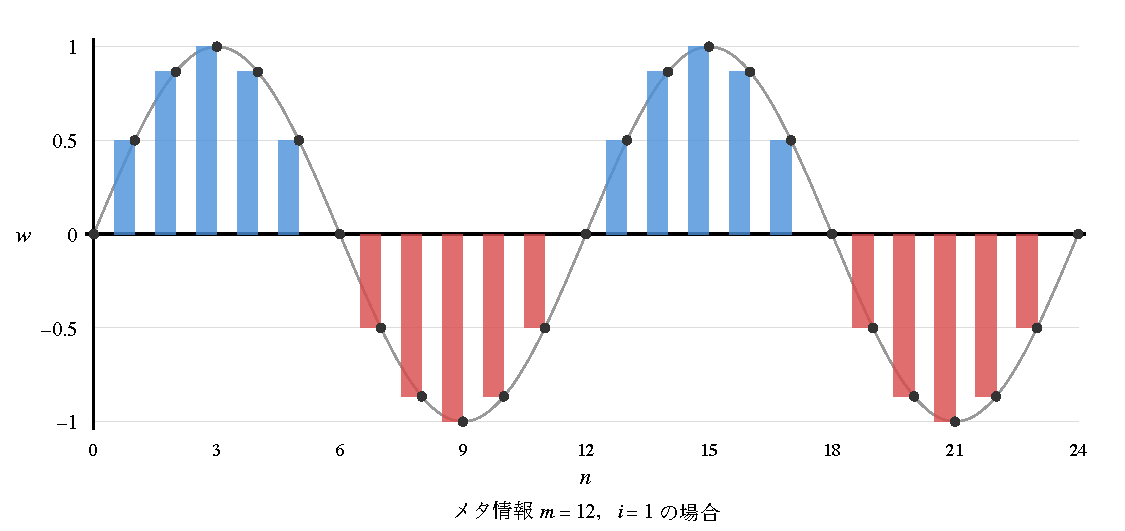
\includegraphics[width=0.8\textwidth]{fig7_sine_wave_sequence.pdf}
  \caption{クラス $B$ の振動シーケンス（メタ情報 $m = 12$，$i = 1$ の場合）}
  \label{fig:sine_wave_sequence}
\end{figure}

棒グラフは各ディレイ回数 $n$ における離散的な出力 $w$ を示し，細線は連続的な正弦波を示す．

\section{縦波の実現}

\subsection{縦波のクラス $C$ の定義}

縦波を実現するクラス $C$ を定義する．クラス $C$ の情報，メタ情報，演算ファンクション $*$ の構造は，クラス $B$（\S 3.4）と全く同一である．

\begin{itemize}
  \item \textbf{クラス $C$ の情報}：スカラー値 $i$，実数値 $w$
  \item \textbf{メタ情報}：カウンタ $n$，波長に相当するディレイ回数 $m$
  \item \textbf{演算ファンクション $*$}：$w = i \cdot \sin(n / m \cdot 360{}^\circ)$
\end{itemize}

クラス $B$ との違いは，出力 $w$ の解釈のみである．クラス $B$ では $w$ を伝播方向に垂直な変位（横波）として扱ったが，クラス $C$ では $w$ を\textbf{伝播方向の変位}として扱う．すなわち，各 $F_D$ の基準位置からの横軸方向のずれとして $w$ を解釈する．

\subsection{縦波の可視化}

開いた縄モデルにクラス $C$ を適用した場合，各 $F_D$ は基準位置から $w$ だけ伝播方向にずれる．これにより，棒が密集する領域（密）と疎になる領域（疎）が交互に現れ，縦波の疎密パターンが得られる．

\begin{figure}[htbp]
  \centering
  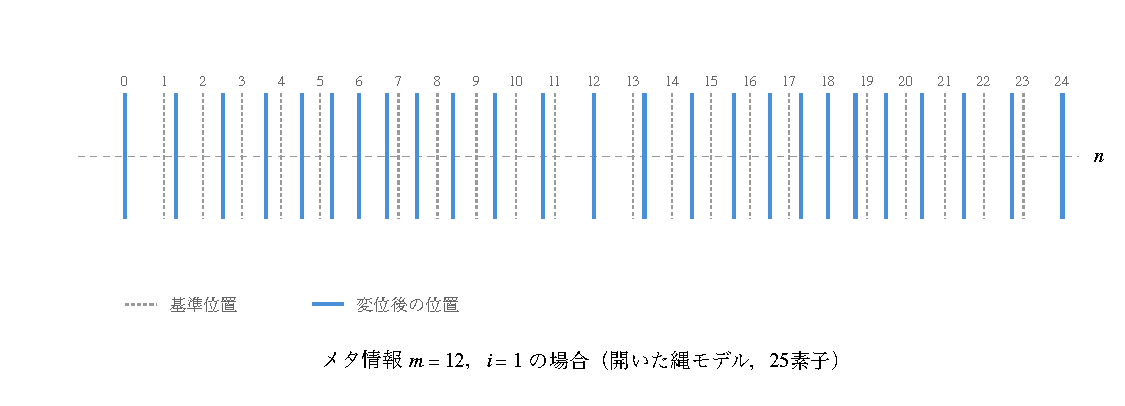
\includegraphics[width=0.8\textwidth]{fig8_longitudinal_wave.pdf}
  \caption{クラス $C$ による縦波の疎密パターン（メタ情報 $m = 12$，$i = 1$ の場合）}
  \label{fig:longitudinal_wave}
\end{figure}

破線は各 $F_D$ の基準位置，実線は $w$ による変位後の位置を示す．

\section{旋回波の実現}

\subsection{旋回波のクラス $D$ の定義}

旋回波を実現するクラス $D$ を定義する．クラス $D$ の情報およびメタ情報の構造は，クラス $B$（\S 3.4）と全く同一である．

\begin{itemize}
  \item \textbf{クラス $D$ の情報}：スカラー値 $i$，実数値 $w$
  \item \textbf{メタ情報}：カウンタ $n$，波長に相当するディレイ回数 $m$
\end{itemize}

クラス $B$ との違いは，演算ファンクション $*$ と出力 $w$ の解釈のみである．

\textbf{演算ファンクション $*$：}

\begin{equation}
w = \frac{n}{m} \cdot 360{}^\circ \mod 360{}^\circ
\end{equation}

出力 $w$ を\textbf{角度}として解釈する．$F_D$ を通過するたびに $n$ がインクリメントされ，$w$ が更新される．$w$ は $0{}^\circ$ から $360{}^\circ$ まで一定の増分で進行し，$360{}^\circ$ に達すると $0{}^\circ$ に戻る．

\subsection{クラス $D$ の振動シーケンス}

$i = 1$，$m = 12$ の場合，単振動回路における $F_D$ の出力 $w$（角度）の遷移を以下に示す．

\begin{table}[htbp]
  \centering
  \begin{tabular}{cc}
    \toprule
    ディレイ回数 $n$ & $w = (n/m \cdot 360{}^\circ) \mod 360{}^\circ$ \\
    \midrule
    0  & $0{}^\circ$ \\
    1  & $30{}^\circ$ \\
    2  & $60{}^\circ$ \\
    3  & $90{}^\circ$ \\
    4  & $120{}^\circ$ \\
    5  & $150{}^\circ$ \\
    6  & $180{}^\circ$ \\
    7  & $210{}^\circ$ \\
    8  & $240{}^\circ$ \\
    9  & $270{}^\circ$ \\
    10 & $300{}^\circ$ \\
    11 & $330{}^\circ$ \\
    12 & $0{}^\circ$ \\
    13 & $30{}^\circ$ \\
    14 & $60{}^\circ$ \\
    $\vdots$ & $\vdots$ \\
    \bottomrule
  \end{tabular}
\end{table}

$n = 12$ で1周（$360{}^\circ$）が完了し，以降は同じパターンを繰り返す．出力 $w$ を角度として解釈すれば，これは一定の角速度で旋回する運動である．

\section{結論}

前稿~\cite{ref2}で導入したスーパークラス，メタ情報，演算ファンクション $*$ の枠組みを用いて，横波（正弦波），縦波，旋回波を実現するクラス $B$, $C$, $D$ を定義した．以下に各クラスの対応を整理する．

\begin{table}[htbp]
  \centering
  \begin{tabular}{clllll}
    \toprule
    クラス & 情報 & メタ情報 & 演算 $*$ & 出力 $w$ の解釈 & 実現する波動 \\
    \midrule
    $A$ & $i$ & $\mathrm{null}$ & $\mathrm{null}$ & --- & 矩形波 \\
    $B$ & $i$, $w$ & $n$, $m$ & $w = i \cdot \sin(n/m \cdot 360{}^\circ)$ & 伝播方向に垂直な変位 & 横波（正弦波） \\
    $C$ & $i$, $w$ & $n$, $m$ & $w = i \cdot \sin(n/m \cdot 360{}^\circ)$ & 伝播方向の変位 & 縦波 \\
    $D$ & $i$, $w$ & $n$, $m$ & $w = (n/m \cdot 360{}^\circ) \!\!\mod 360{}^\circ$ & 角度 & 旋回波 \\
    \bottomrule
  \end{tabular}
\end{table}

いずれの場合も，ディレイ回路 $F_D$ およびNOT演算回路の定義（\cite{ref1} \S 2.2〜\S 2.4）は一切変更していない．クラスの情報と演算ファンクション $*$ の選択のみで，矩形波を含む4種類の波動パターンが構成できることを示した．

\begin{thebibliography}{9}
\bibitem{ref1} 木原範昭「情報伝達の情報論的整理」研究ノート，2026年4月．
\bibitem{ref2} 木原範昭「ディレイ回路モデルに内在する対称性の整理」研究ノート，2026年4月．
\end{thebibliography}

\end{document}
